\section{Alert Production}
\label{sec:ap}



Alert Production is run each night to product catalogs and images for sources that have varied or moved relative to a previous observation.  The data products produced by Alert production are given in  table~\hyperref[table:ap_data_products].

\begin{table}
\small
\begin{tabularx}{\textwidth}{ | l | l | X | }
  \hline
  {\bf Name} & {\bf Availability} & {\bf Description} \\
  \hline
  DIASource & Stored &
  Measurements from difference imagine analysis of individual exposures. \\
  \hline
  DIAObject& Stored &
  Aggregate quantities computing by associating spatially colocated DIASources. \\
  \hline
  DIAForcedSource & Stored &
  Flux measurements on each difference image at the position of every DIAObject. \\
  \hline
  SSObject & Stored &
  Solar system objects derived by associating DIASources and inferring their orbits. \\
  \hline
  CalExp & Stored &
  Calibrated exposure images for each CCD/visit (sum of two snaps). \\
  \hline
  DiffExp & Stored &
  Difference between CalExp and PSF-matched template coadd. \\
  \hline
\end{tabularx}
\caption{Table of derived and persisted data products produced during a Alert Production.  A description of these data products can be found in the Data Products Definition Document (LSE-163).
\label{table:ap_data_products}}
\end{table}


Alert Production is designed as five separate components: single frame
processing, alert detection, alert generation, precovery photometry,
and a moving objects pipeline. The first four of these components run
as a linear pass through of the data. The moving objects pipeline is
run independently of the rest of the alert production. The flow of
information through this system is shown in figure~\ref{fig:nightly}.

\begin{figure}[th]
\begin{center}
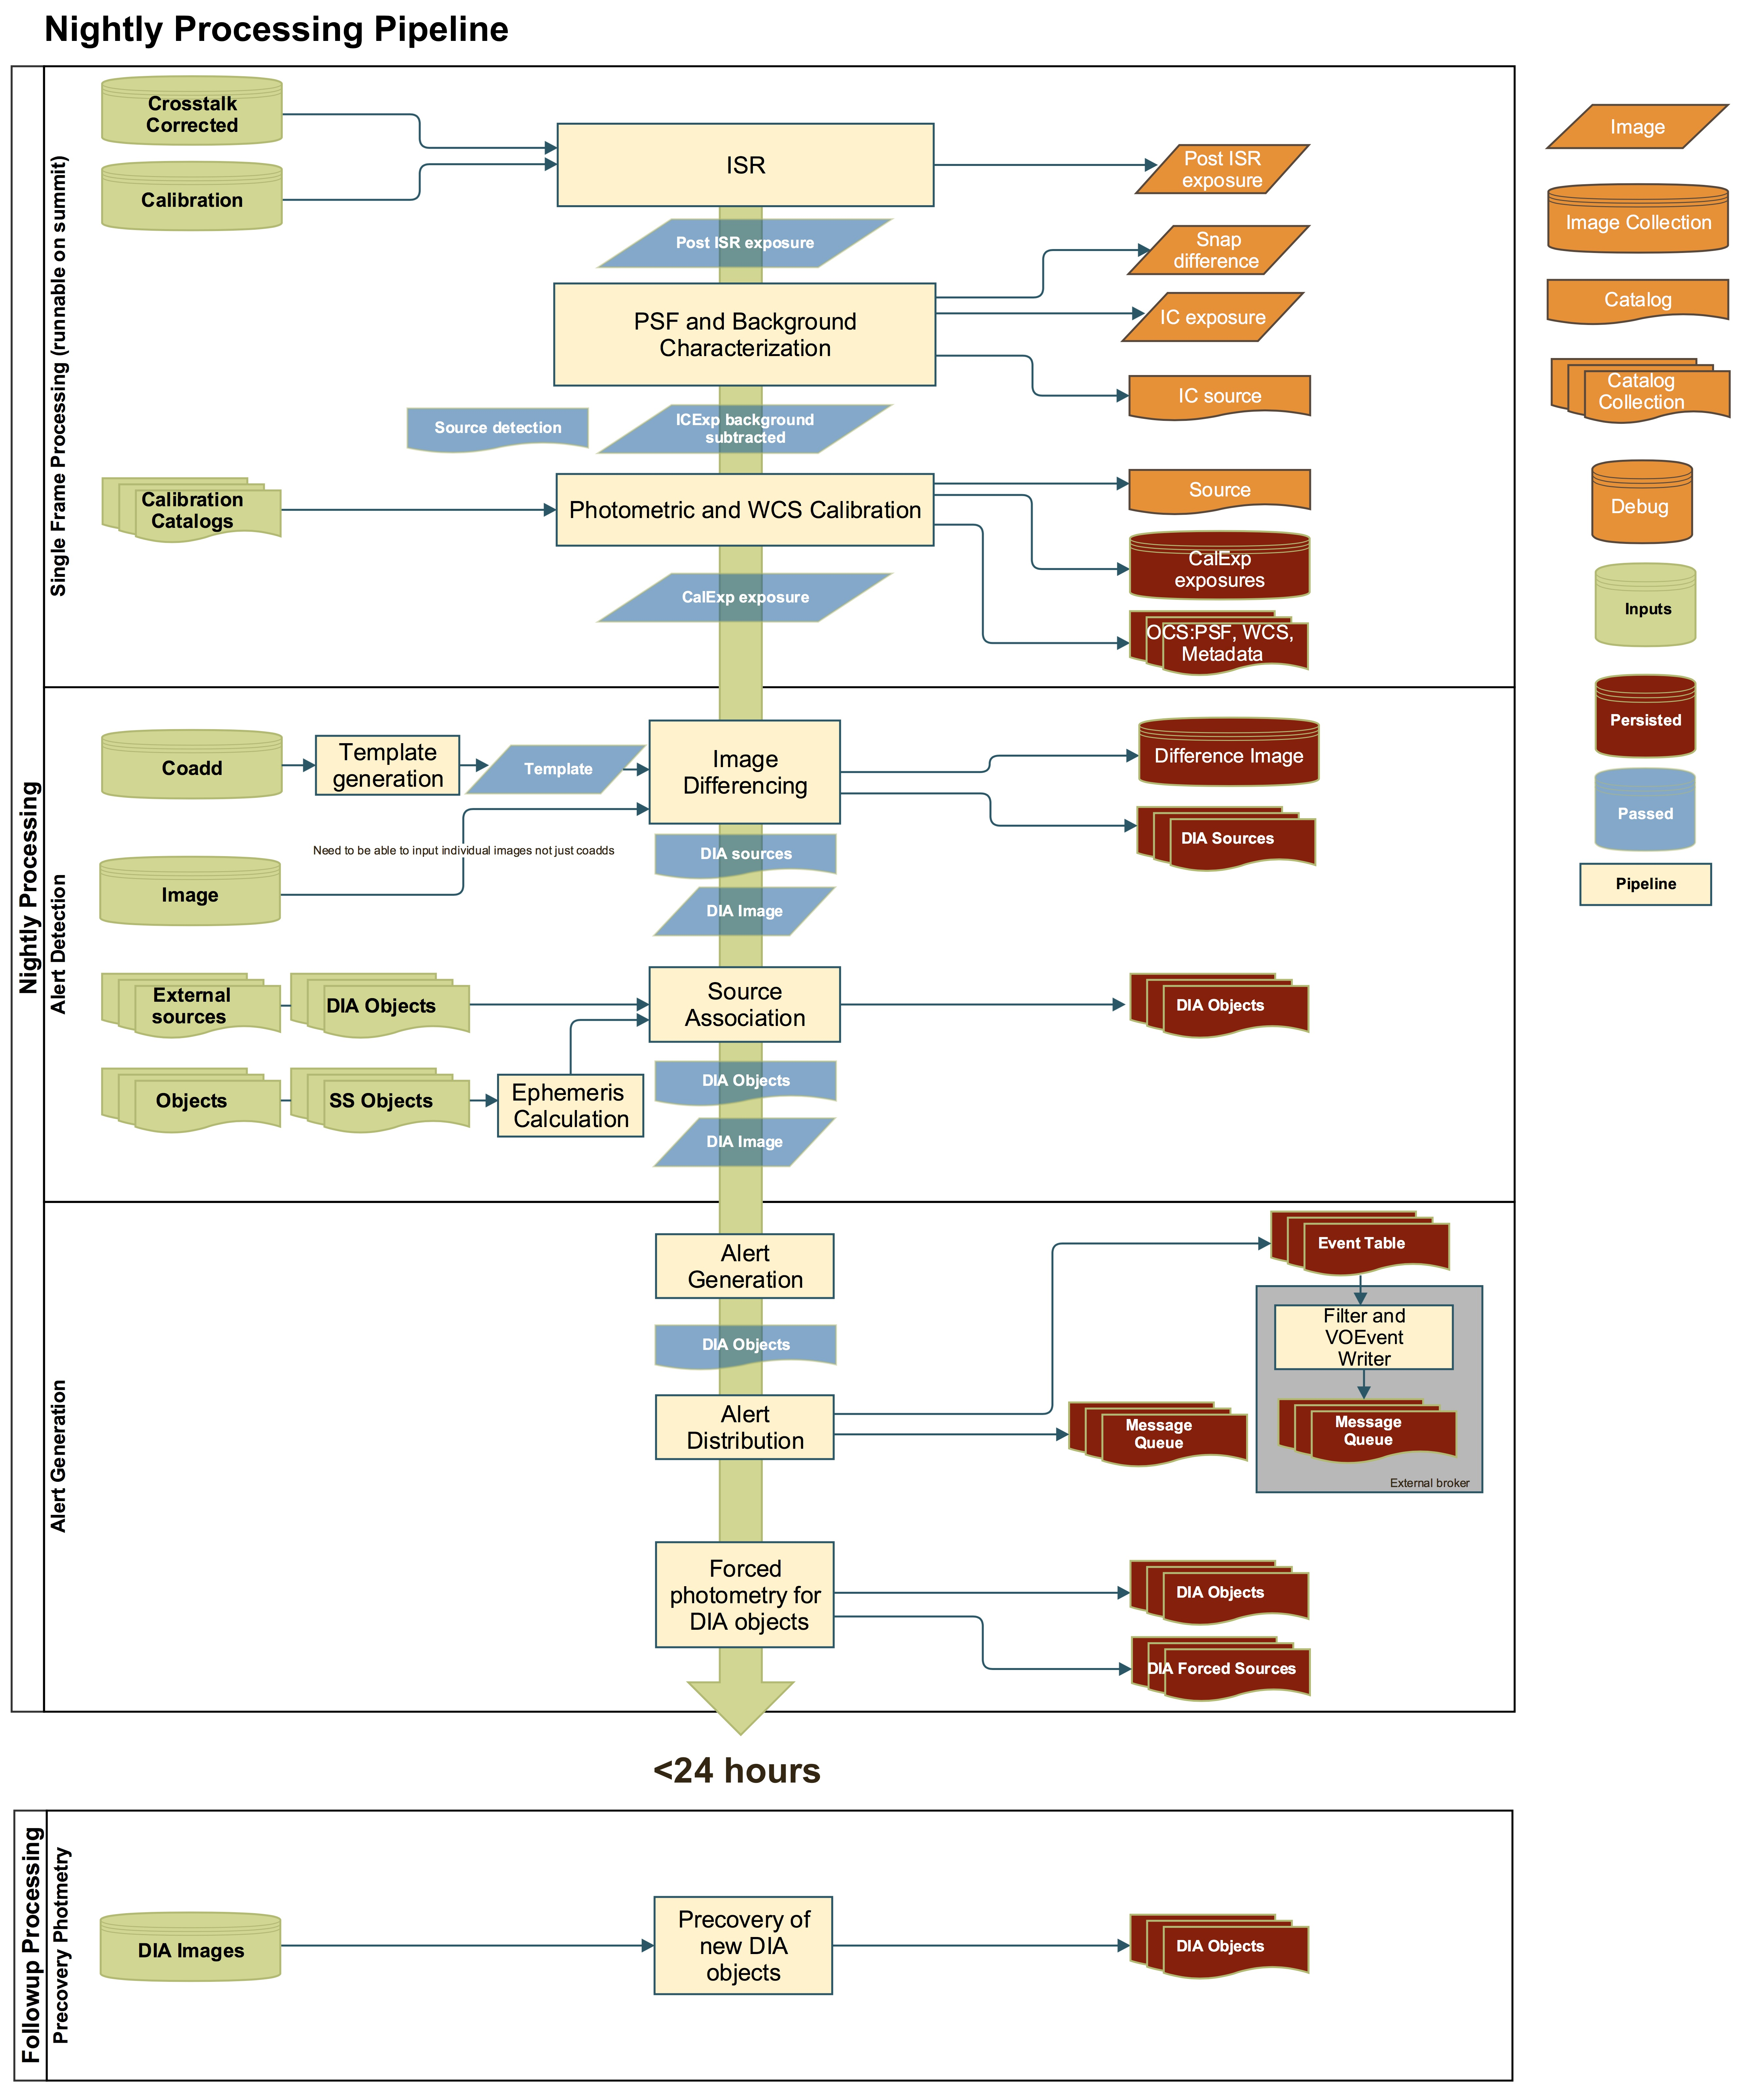
\includegraphics[width=0.9\textwidth]{figures/Level_1_Processing_Flowchart.jpg}
\caption{\label{fig:nightly} The alert production flow of data through
  the processing pipelines (single frame processing, alert detection,
  alert generation, precovery photometry) }
\end{center}
\end{figure}

In this document we do not address the question of estimating the selection function for the alert generation through the injection of simulated sources. Such a process could be undertaken in a parallel processing string that starts from the generation of the CalExp images though, given the available computational resources, this would likely only be able to sample the selection function over a subset

\subsection{Single Frame Processing Pipeline (\wbsSFM)}
\label{sec:apSingleFrameProcessing}

Single Frame Processing (SFM) Pipeline is responsible for reducing raw or camera corrected image data to \emph{calibrated exposures}, the detection and measurement of \Sources (using the components functionally a part of the Object Characterization Pipeline), the characterization of the point-spread-function (PSF), and the generation of an astrometric solution for an image.

Single Frame Processing pipeline will be implemented as a flexible   framework where new processing steps can be added without modifying the stack code. It should be possible for this pipeline or a subset of this pipeline  to be run at the telescope facility during commissioning and operations.  

\paragraph{Input Data: Raw}

Amplifier images that the camera has corrected for crosstalk, overscan, linearity.  All images from a visit should be available to the task (including snaps). An approximate WCS is assumed to be available as metadata

\paragraph{Input Data Product: Reference}

A full-sky reference catalog of stars derived either from an external survey (e.g.\ Gaia) or from the Data Release Processing.

Flatfield calibration images for all passbands and all CCDs appropriate for the time at which the observations were undertaken

List of the positions and extents of sensor defects for all CCDs within the focal plane

Metadata for all CCDs including electronic parameters (saturation limits, readnoise, electronic footprint)

\paragraph{Output Data Product: CalExp}

A calibrated exposure (CalExp).  CalExp is an \hyperref[sec:spImagesExposure]{Exposure} object. The CalExp will contain a PSF, WCS, PhotoCalib and Background. The pixel data will include the image, mask, and variance. 

\paragraph{Output Data Product: Source}

A catalog of Sources with measured features (as described in \ref{sec:ac}). 


\paragraph{Output Data Product: Metadata}
A parameterization of the PSF for the visit, the WCS for the visit,
and associated metadata (e.g.\ photometric depth) must be made
available to the telescope Observatory Control System (OCS). It is
expected that these data will be persisted within a database that will
be queried by the OCS.


SFM pipeline functions include:
\begin{itemize}
\item Assembly of per-amplifier images to an image of the entire CCD;
\item Instrumental Signature Removal;
\item Cosmic ray rejection and snap combining;
\item Per-CCD determination of zeropoint and aperture corrections;
\item Per-CCD PSF determination;
\item Per-CCD WCS determination and astrometric registration of images;
\item Per-CCD sky background determination;
\item Source detection and measurement on single frame images
\item Generation of metadata required by the OCS
\end{itemize}

Calibrated exposure produced by the SFM pipeline must possess all information necessary for measurement of source properties by single-epoch Object Characterization algorithms.

\paragraph{Actions in case of failure:}

In the case camera data are not available due to a network outage that is longer than the data buffer at the summit the single frame processing will work on raw images (i.e.\ without the camera pixel corrections) and be run in a batch mode. 



\paragraph{Instrumental Signature Removal:}~
\label{sec:apISR}
Instrumental Signature Removal characterizes, corrects, interpolates
and flags the camera (or raw) images to generate a flat-fielded and corrected
exposure.

\paragraph{Pipeline Tasks}
\begin{itemize}
\item Mask CCD defects based on the and saturation
\item Assembly
\item Full frame corrections: Dark, Flats (includes fringing)
\item Pixel level corrections: Brighter fatter, static pixel size effects
\item Interpolation of defects and saturation
\item \hyperref[sec:artifact]{CR rejection}
\item Generate snap difference
\item Snap combination
\end{itemize}


\paragraph{PSF and background determination:}~
\label{sec:apPSFBackground}

Given exposures that have been processed through the Instrument Signature Removal, sources must be detected that will be used to determine the WCS and photometric calibration of the images. Detection and measurement of the properties of these calibration Sources requires knowlege of the PSF and background for the image which in turn requires knowledge of the sources on the image. An iterative procedure is, therefore, adopted to generate the Source catalog. 

\paragraph{Pipeline Tasks}
The procedure for PSF and background estimation and the associated
algorithmic components. Convergence criteria for the procedure is not
defined but the default procedure assumes three iterations.
\begin{itemize}
\item \hyperref[sec:acBackgroundEstimation]{Background estimation}
\item \hyperref[sec:acSourceDetection]{Source detection} to the 5$\sigma$ limit of
%\item Single CCD \hyperref[sec:acDeblending]{Deblend sources}
\item Selection of PSF candidate stars based on a signal-to-noise threshold 
  (default 50 $\sigma$) and isolated sources 
\item Single CCD \hyperref[sec:acSingleCCDPSF]{PSF determination} given the selected bright sources
%\item Single CCD \hyperref[sec:acModelSpatialPSF]{PSF spatial model}
\end{itemize}


\paragraph{Source measurement:}~
\label{sec:apSourcemeasurement}

For the Source catalog generated in \label{sec:apPSFBackground} measure the source properties using a subset of features measured in \label{sec:drpMeasureSources}. Source measurement if for all sources within the Source catalog and not just the bright subset used to calibrate the PSF. 

\paragraph{Pipeline Tasks}
We anticipate using the following plugin algorithms for \label{sec:drpMeasureSources}
\begin{itemize}
\item \hyperref[sec:acCentroidAlgorithms]{Centroids}
\item \hyperref[sec:acPixelFlags]{Pixel Flag Aggregation}
\item \hyperref[sec:acAperturePhotometry]{Aperture Photometry} (but only for one or two radii) 
\item \hyperref[sec:acPSFPhotometry]{PSF Photometry} 
\item \hyperref[sec:acStaticPointSourceModels]{Static Point Source Models}
\item  \hyperref[sec:apertureCorrection]{Aperture correction} for  detected sources
\end{itemize}

\paragraph{Photometric and Astrometric calibration:}~
Photometric and astrometric calibration entails a ``semi-blind'' cross match of a reference catalog (derived either from the DRP Objects or from an external catalog), the generation of a WCS (on the scale of a CCD or visit), and the generation of a photometric zeropoint (on the scale of a CCD).

\paragraph{Pipeline Tasks}
Photometric and astrometric calibration performed at the scale of a
single sensor (extended to the scale of a visit depending on required fidelity)
\begin{itemize}
\item CCD level \hyperref[sec:acSingleCCDReferenceMatching]{source
    association} between the DRP reference catalog and Sources from the \ref{sec:apSourcemeasurement}
\item Generation of a \hyperref[sec:acSingleCCDPhotometricFit]{photometric solution} at the level of a single CCD
\item Decomposition of the astrometric components (e.g.\ optical distortions, sensor tree-rings) for a single CCD and generation of an \hyperref[sec:acSingleCCDAstrometricFit]{astrometric fit} at the level of a single CCD
\item Persistence of the astrometric, PSF, and photometric solutions so that the OCS can incorporate it into their telemetry
\end{itemize}

Given the number of stars available on a CCD or the complexity of the astrometric solutions for the LSST it may be necessary that the astrometric and photometric solutions must be performed at the level of a visit and not a CCD.  For these cases the operations will be \hyperref[sec:acSingleVisitReferenceMatching]{single visit matching},   \hyperref[sec:acSingleCCDPhotometricFit]{single visit photometric solutions}, \hyperref[sec:acSingleVisitAstrometricFit]{single visit astrometric fits}.

Astrometric and photometric performance within crowded fields will require that the order of the WCS should depend on the number of calibration Sources that are available.

\subsection{Alert Detection (\wbsDiffim)}
\label{sec:apAlertDetection}

Alert Detection identifies variable, moving, and transient sources within a calibrated exposure by subtracting a deeper template image. Sources, DIASources, detected on a DIAImage are associated with known Objects (including SSObjects that have been propagated to the date of the CalExp exposure) and their properties measured. The resulting DIAImages and DIAObjects will be persisted by the Alert Detection pipeline.

Alert Detection pipeline shall difference, and detect and characterize sources in the time required to achieve the 60 second design goal for nightly processing (current timing allocation: 24 seconds). The algorithms employed by the pipeline shall result in purity and completeness of the sample as required by the \DMSR\@. Image differencing shall perform as well in crowded as in uncrowded fields. 


\paragraph{Input Data: CalExp}

Calibrated exposure processed through \ref{sec:apSingleFrameProcessing} with associated WCS, PSF, mask, variance, and background estimation.

\paragraph{Input Data: Coadd}

TemplateCoadd images that spatially overlap with the CalExp images processed through \ref{sec:apSingleFrameProcessing}. This Coadd image is optimized for image subtraction and is expected to be characterized in terms of a tract/patch/filter. Generation of this template may account for differential chromatic refraction or be generated for a limited range of airmass and seeing.

\paragraph{Input Data Product: Object}

Objects that spatially overlap with the CalExp images processed through \ref{sec:apSingleFrameProcessing}. This Object catalog will provide the source list for determining nearest neighbors to the detected DIASources. 

Flatfield calibration images for all passbands and all CCDs appropriate for the time at which the observations were undertaken 

\paragraph{Input Data Product: DIAObjects}

DIAObjects that spatially overlap with the CalExp images processed through \ref{sec:apSingleFrameProcessing}. This DIAObject catalog will provide the association  list against which the DIASources will be matched. 

\paragraph{Input Data Product: SSObjects}

The SSObject list at the time of the observation. The SSObject positions will be propagated to the date of the CalExp observations and will provide an association  list for cross-matching against the DIASource list to identify known Solar System objects.

\paragraph{Input Data Product: Reference}

Classification of DIASources based on their morphological features (and possibly estimates of the local density or  environment associated with the DIASource) will be undertaken prior to association in order to reduce the number of false positives. The data structures that define these classifications will be required as an input to the spuriousness analysis. 

\paragraph{Output Data Product: DIAImage}

Image differences (DIAImage) derived from subtracting a CalExp from a TemplateCoadd image 

\paragraph{Output Data Product: DIASource}

Sources detected and measured from the DIAImages (DIASources) using the set of parameters described in table \hyperref[table:ap_features] will be persisted


\paragraph{Output Data Product: DIAObject}

DIASource will be associated with existing DIAObjects and persisted. New DIASource (i.e.\ those not persisted) will generate a new instance of a DIAObject 

\paragraph{Output Data Product: DIAForcedPhotometry}

For all DIAObjects forced photometry will be undertaken given a time windowed estimate of the DIAObject position.


The process for image differencing requires the following steps
\begin{itemize}
\item Creation or \hyperref[sec:acRetrieveTemplate]{retrieval} of a TemplateCoadd.
\item Matching the astrometry and PSF of a CalExp to the TemplateCoadd and subtracting the template image from the CalExp. This will require accounting for the relative differences in image quality and noise between the template and CalExp.
\item Removal of spurious DIASources 


\item \hyperref[sec:acWarping]{Warping or resampling} of the TemplateCoadd to match the WCS of the CalExp. It is possible that the an operation to astrometrically match the TemplateCoadd and CalExp using faint source will need to be undertaken dependent on the accuracy of the WCS.
\item For CalExp images with an image quality that is better than the TemplateCoadd preconvolve the CalExp image with the PSF use a  \hyperref[sec:spKernels]{convolution kernel}. This reduces the significance of any deconvolution in the PSF matching.
\item Match the CalExp and TemplateCoadd image and  \hyperref[sec:acImageSubtraction]{subtract} the images to generate a DIAImage
\item \hyperref[sec:acDiffImDecorrelation]{Decorrelate} the DIAImage to reduced the correlations in the noise due to the convolution with the image differencing matching kernel. 
\item \hyperref[sec:acSourceDetection]{Detect DIAsources} on the DIAImage. Convolution with a detection kernel will depend on whether the CalExp was preconvolved in step 3
\item (optional) Dependent on the source density \hyperref[sec:acSingleFrameDeblending]{single frame deblending} will split \hyperref[sec:spFootprints]{Footprints} with multiple peaks into deblend families.
\item \hyperref[sec:acDiffImMeasurement]{ Measure sources} on the DIAImage including \hyperref[sec:acDipoleModels]{dipole models}. The specific algorithms used for measurement of DIASources will depend on whether the CalExp image was preconvolved.
\item \hyperref[sec:acSpuriousnessAlgorithms]{Spuriousness algorithms} also known as ``real-bogus'' may have to be applied at this time dependent on the number of false positives. DIASources classified as spurious at this stage may not be persisted (dependent on the density of the false positives)
\item \hyperref[sec:acDIAObjectGeneration]{Source association} will be undertaken for all DIASources. Matching will be to DIAObjects, Objects, and the propagated positions of SSObjects. Positions for DIAObjects will be based on a a time windowed average of the DIASources that make up the DIAObject. A probabilistic association will need to account for one-to-many and many-to-one associations. It may be necessary to generate joint associations across all DIAObjects (and associated DIASources) in the local  vicinity of a DIASource to correct for mis-assignment from previous observations. All unassociated DIASources will instantiate a new DIAObject
\item \hyperref[sec:acForcedMeasurement]{Forced measurement} will be run for all DIAObjects on the DIAImage

\end{itemize}



\label{sec:acDCRTemplates}

\paragraph{Template Generation}~

Template generation requires the creation or \hyperref[sec:acRetrieveTemplate]{retrieval} of a TemplateCoadd w that is matched to the position and spatial extent of the input CalExp. Generation of the TemplateCoadd could be from a persisted Coadd that was generated from CalExp exposures with comparable (within a predefined tolerance) airmass and parallactic angles or from a model that corrects for the effect of  \hyperref[sec:acDCRTemplates]{differential chromatic refraction}. It is expected that these operations would be undertaken on a CCD level but for efficiency the TemplateCoadd might be returned for a full visit. 


\paragraph{Pipeline Tasks}
\begin{itemize}
\item Query for a TemplateCoadd images that are within a given time interval of the CalExp  (default 2 years) of the current sensor image, and are within a specified airmass and parallactic angle
\item (optional) Derive an airmass and DCR corrected TemplateCoadd from a model (see  \hyperref[sec:acDCRTemplates]{ DCR template generation}). The direction of the DCR correction will be aligned with the 
  ``parallactic angle'' of the CalExp image
\end{itemize}

\paragraph{Image differencing}~

Image differencing incorporates the matching of a CalExp to a TemplateCoadd (astrometrically and in terms of image quality), subtraction of the tempalte image, detection and measurement of DIASources, removal of spurious DIAsources, and association of the DIASources with previously identified DIAObjects, Objects, and SSObjects. 

\paragraph{Pipeline Tasks}
\begin{itemize}
\item Determine a relative astrometric solution from the WCS of the TemplateCoadd image and CalExp image
\item Match \hyperref[sec:apSourcemeasurement]{DRP} sources for the TemplateCoadd against sources from \hyperref[sec:apSingleFrameProcessing]{SFP} of the raw images 
\item \hyperref[sec:acWarping]{Warp or resample} the TemplateCoadd to match the astrometry of the CalExp. It is possible that the an operation to astrometrically match the TemplateCoadd and CalExp using faint source will need to be undertaken dependent on the accuracy of the WCS.
\item For CalExp images with an image quality that is better than the TemplateCoadd preconvolve the CalExp image with the PSF use a  \hyperref[sec:spKernels]{convolution kernel}. This reduces the significance of any deconvolution in the PSF matching.
\item \hyperref[sec:acDiffImDecorrelation]{Match} the PSF of the CalExp and TemplateCoadd images and construct a spatial model for the matching kernel
\item Apply the matching kernel and \hyperref[sec:acImageSubtraction]{subtract} the images to generate a DIAImage
\item \hyperref[sec:acDiffImDecorrelation]{Decorrelate} the DIAImage to reduced the correlations in the noise due to the convolution with the image differencing matching kernel. 
\item \hyperref[sec:acSourceDetection]{Detect DIAsources} on the DIAImage. Convolution with a detection kernel will depend on whether the CalExp was preconvolved in step 3
\item \hyperref[sec:acDiffImMeasurement]{ Measure sources} on the DIAImage including \hyperref[sec:acDipoleModels]{dipole models}. The specific algorithms used for measurement of DIASources will depend on whether the CalExp image was preconvolved.  Source measurements will include: \hyperref[sec:acDipoleModels]{dipole fit}, \hyperref[sec:acTrailedPointSourceModels]{trailed source} measurement
\item Measure flux on snap difference for all DIASources
\item \hyperref[sec:acSpuriousnessAlgorithms]{Spuriousness algorithms} also known as ``real-bogus'' may have to be applied at this time dependent on the number of false positives. DIASources classified as spurious at this stage may not be persisted (dependent on the density of the false positives). The default technique will be based on a trained random forest classifier. It is likely that the training of this classifier will need to be conditioned on the image quality and airmass of the observations.
\end{itemize}

\paragraph{Source Association}~

In Source Association DIASources detected within a given CCD will be cross-matched (\hyperref[sec:acDIAObjectGeneration]{associated}) with the DIAObject table and the SSObjects (whose ephemerides have been generated for the time of the current observation. The association will be probabilistic  and account for the uncertainties within the positions. Dependent on the available computational resources the association may include flux and priors on expected proper motions for the sources. External targets (e.g.\ well resolved transient events from other telescopes or instruments) can be incorporated within this component of the nightly pipeline enabling either matching to DIASources or generation of forced photometry at the position of the external source. It is not clear that this is an objective of the pipeline. 


\paragraph{Pipeline Tasks}
\begin{itemize}
\item The \hyperref[sec:acEphemerisCalculation]{ephemerides} for SSObjects will be generated for those sources overlapping a DIAImage
\item \hyperref[sec:acDIAObjectGeneration]{Source association} will be undertaken for all DIASources. Matching will be to DIAObjects, and the ephemerides of SSObjects. Positions for DIAObjects will be based on a a time windowed average of the DIASources that make up the DIAObject. A probabilistic association will need to account for one-to-many and many-to-one associations. It may be necessary to generate joint associations across all DIAObjects (and associated DIASources) in the local  vicinity of a DIASource to correct for mis-assignment from previous observations. This could include the pruning and reassignment of DIASources between DIAObjects.
\item DIASources will be \hyperref[sec:acDIAObjectGeneration]{associated} with the Object table from DRP. In its simplest case this will be a nearest neighbor search that will define a set of nearest neighbors (the default radius for association is not defined) that will be persisted with DIAObjects as a measure of local environment. More sophisticated association may be undertaken to match the DIASources to Objects in order to enable access to the DRP properties of a source (e.g.\ proper motion and parallax - see below).
\item DIASources unassociated with a DIAObject will instantiate a new DIAObject
\item The agregate positions for the DIAObjects will be updated based on a rolling time window (default 30 days). 
\item (optional) The proper motion and parallax will be \hyperref[sec:acStellarMotionFitting]{updated}. It is not currently clear if there is a science case for generating proper motions and parallaxes within the DIAObjects if the DRP Objects are available for each source. 
\end{itemize}


\subsubsection{Prototype Implementation}

The prototype code is available at \url{https://github.com/lsst/ip_diffim}. The current prototype, while functional, will require a partial redesign to be transfered to construction to address performance and extensibility concerns.

\clearpage

\subsection{Alert Generation Pipeline (\wbsAP)}

\subsubsection{Key Requirements}

Alert Generation Pipeline shall take the newly discovered \DIASources and all associated metadata as described in the \DPDD, and deliver alert packets in \VOEvent format to a variety of endpoints via standard IVOA protocols (eg., VOEvent Transport Protocol; VTP\@).

To directly serve the end-users, the Alert Generation Pipeline shall provide a basic, limited capacity, alert filtering service. This service will run at the LSST U.S. Archive Center (at NCSA). It will let astronomers create simple filters that limit what alerts, and what fields from those alerts, are ultimately forwarded to them. These \emph{user defined filters} will be possible to specify using an SQL-like declarative language, or short snippets of (likely Python) code.

Since there is a need to keep both the alert database and the brokers consistent, there is a big win if both the database and the brokers read from the same fault tolerant intermediate persistence format.  A redundant, cluster based, strongly ordered, message system like Kafka (http://kafka.apache.org) is a very attractive option as the intermediate persistence.  It is very similar in concept to persisting to some well known file format with the addition of reduntant storage, configurable expiration time of messages, and strict ordering so database catch-up is trivial.  It is also scalable.


\paragraph{Input Data: Object}

DIAObjects that generated through image differencing and association will be used to generate alert packets 

\paragraph{Input Data: CalExp}

The CCD level CalExp will be used to generate postage stamp or cut out images of DIAObjects  within the CCD

\paragraph{Input Data: TemplateCoadd}

The TemplateCoadd used in the image subtraction will be used to  generate postage stamp or cut out images of DIAObjects   within the CCD


\paragraph{Input Data Product: DIAImage}

The image subtracted DIAImage will be used to  generate postage stamp or cut out images of DIAObjects within the CCD

\paragraph{Output Data Product: VOevents}

VOEvents generated from the DIAObjects will be persisted. The form of these persisted events has  not been decided.

\paragraph{Alert generation}~

\paragraph{Pipeline Tasks}
 \begin{itemize}
\item Generate postage stamps for all DIASources: direct image and difference image
\item Push alert records to alert persistence
\item Alert database ingestion client reads all new alerts and persists them permanently in the alert database
\end{itemize}

\paragraph{Alert Distribution: To community brokers}

\paragraph{Pipeline Tasks}
\begin{itemize}
\item For each visit read all new alert records from the alert persistence
\item Package each message as a properly formatted VOEvent
\item Bundle VOEvents using a pre-negotiated format
\item Transmit bundled VOEvents to community broker endpoints
\end{itemize}

\paragraph{Alert Distribution: Minimal brokers}
\noindent
Each minimal broker will have some subset of users.  The following is for a single broker.

\paragraph{Pipeline Tasks}
\begin{itemize}
\item Read new alert records from the alert persistence in order
\item Filter event records for relevance (WHERE)
\item Filter event columns for content (SELECT)
\item Package event as a valid VOEvent
\item Publish the VOEvent to the appropriate endpoint (potentially another messaging queue so clients can access asynchronously)
\end{itemize}

\paragraph{Forced Photometry on all DIAObjects}~

\paragraph{Pipeline Tasks}
\begin{itemize}
\item Compute forced photometry on all DIAObjects in the field.  This
  does not end up in the alerts.
\item Update the DIA Object forced photometry tables
\end{itemize}

\subsubsection{Prototype Implementation}

\clearpage

\subsection{Precovery Photometry Pipeline}

\noindent
{\bf Input Data:}\\
\begin{itemize}
\item Butler access to DIA images within finite time interval (default 
  30 days) 
\item Butler access to DIAobjects detected from the previous night 
  with no associations 
\end{itemize}
{\bf Output Data}\\
\begin{itemize}
\item Updated and persisted forced photometry tables for all newly
  detected DIAobjects
\end{itemize}

\subsubsection{Key Requirements}

Within 24 hrs.

\paragraph{Precovery of new DIAObjects}~

\noindent
{\bf Subtasks:}
\begin{itemize}
\item Force photometer in difference images for all new DIAObjects for the past 30 days.
\end{itemize}
\clearpage

\subsection{Moving Object Pipeline (\wbsMOPS)}

\subsubsection{Key Requirements}

The Moving Object Pipeline is responsible for generating and managing the Solar System\footnote{Also sometimes referred to as `Moving Object'} data products. These are Solar System objects with associated Keplerian orbits, errors, and detected \DIASources. Quantitatively, it shall be capable of detecting 95\% of all Solar System objects that meet the findability criteria as defined in the \OSS\@. 

\subsubsection{Baseline Design}
{\bf Input Data}\\
\begin{itemize}
\item 'Orphan' DIASources from the last night of observing.  This means DIASources that are not associated with a DIAObject.  DIASources associated with an SSObject in the night are still passed through the MOPS machinery
\item DIAObject database
\item SSObject database
\item Exposure metadata database
\end{itemize}
{\bf Output Data}\\
\begin{itemize}
\item Updated SSObject databaase
\item Updated DIASource database
\end{itemize}
{\bf Anscillary Products}\\
\begin{itemize}
\item Tracklet database
\item Track database
\item Intermediate orbit prediction database
\end{itemize}
{\bf Actions in case of failure}\\
{\bf Alternative procedures}\\

{\bf Subtasks:}
\begin{itemize}
\item Feed all input orphan DIASources to \hyperref[sec:acMakeTracklets][makeTracklets].
\item Run \hyperref[sec:acAttributionAndPrecovery]{attribution and precovery} on with just the tracklets and DIASources from the previous night.  This culls any tracklets or DIASources that obviously belong to an existing SSObject from the rest of the processing.
\item Compute new \hyperref[sec:acOrbitFitting]{orbits} and \hyperref[sec:acOrbitMerging]{merge orbits}.
\item Run \hyperref[sec:acAttributionAndPrecovery]{attribution and precovery} on with full survey of tracklets and DIASources but only running over new SSObjects.
\item \hyperref[sec:acOrbitMerging]{Merge Orbits}.
\end{itemize}

\subsubsection{Prototype Implementation}

Prototype MOPS codes are available at
\url{https://github.com/lsst/mops_daymops} and
\url{https://github.com/lsst/mops_nightmops}. We expect it will be
possible to transfer a significant fraction of the existing code into
Construction. Current DayMOPS prototype already performs within the
computational envelope envisioned for LSST Operations, though it does
not yet reach the required completeness requirement.


